\documentclass[a4paper,11pt]{book}

% Essential packages
\usepackage[utf8]{inputenc} % UTF-8 encoding
\usepackage[T1]{fontenc}    % Font encoding
\usepackage[english]{babel} % English language
\usepackage{graphicx}       % For including images
\usepackage[version=4]{mhchem} % chemical package
\usepackage{amsmath, amssymb} % Advanced math symbols
\usepackage{hyperref}       % For clickable links
\usepackage{geometry}       % For custom margins
\usepackage{setspace}       % For line spacing
\usepackage{fancyhdr}       % For headers and footers
\usepackage{biblatex}       % For bibliography management
\usepackage{listings}
\usepackage{booktabs}
\usepackage{caption}   % Per personalizzare le didascalie
\usepackage{subcaption} % Per immagini affiancate
\usepackage{array}
\usepackage{colortbl}
\usepackage{xcolor} % Per definire colori personalizzati

\lstset{
    basicstyle=\ttfamily\small,  % Tipo di carattere (monospace)
    keywordstyle=\bfseries,      % Parole chiave in grassetto
    commentstyle=\itshape,       % Commenti in corsivo
    columns=fullflexible,        % Allineamento corretto
    frame=single,                % Bordo intorno al codice
    breaklines=true,             % Andare a capo automaticamente
    captionpos=b                 % Posizione della caption (bottom)
}
% Set margins
\geometry{
    a4paper,
    top=3cm,
    bottom=3cm,
    left=3cm,
    right=3cm,
}

% Line spacing
\onehalfspacing

% Header and footer setup
\pagestyle{fancy}
\fancyhf{}
\fancyhead[L]{\leftmark}
\fancyfoot[C]{\thepage}

% Load bibliography
\addbibresource{bibliography.bib}

\begin{document}
\frontmatter % to use roman page numbering for the index and title page

% Title page
\begin{titlepage}
    \centering
    % Logo
    \begin{figure}[h]
        \centering
        
\includegraphics[width=\linewidth]{tesiSCIENZE_TECNOLOGIE.jpg}
    \end{figure}
    
    {\scshape\Large Dipartimento di Fisica \\ Corso di Laurea Magistrale in Fisica\par}
    \vspace{1.5cm}
    {\Huge\bfseries  Numerical Solutions of frequency dependence of real and 
        imaginary parts of the complex conductivity in Eliashberg theory\par}
    \vspace{2cm}
    
    % Informazioni sul relatore e correlatore a sinistra
    \begin{flushleft}
      {\Large Supervisor: \par}
      {\Large Co-supervisor: \par}
    \end{flushleft}
    
    %\vfill
    
    % Informazioni sull'autore e matricola in basso a destra
    \begin{flushright}
      {\Large Thesis author: \\ Enrico Vianelli\par}
      {\Large Matr. \par} 
    \end{flushright}
    \vfill
    {\Large Accademic year 2025/2026\par}
\end{titlepage}

\chapter*{Introduction}

\tableofcontents

\mainmatter % end of roman page numbering


\chapter{BCS theory}

...BCS SHORT REVIEW

\section{Mattis Bardeen formula}

The Mattis-Bardeen formula (MB) describes the complex conductuvity $\sigma(\omega, T)$ of superconductors in the 
BCS theory framework, so it is accurate for weak-coupling superconductors materials.
The originally form was derived by Mattis and Bardeen in 1958, and also assumes the clean
limit $l\rightarrow\infty$ and the Pippard limit $\xi \leq \lambda_L$. Then Nam showed in 1967 that
the formula is valid also in the dirty limit $l\rightarrow 0$ and the local limit $\xi \gg \lambda_L$.
\\
The MB equations are given by the two integrals
\begin{equation}
    \begin{split}
        \frac{\sigma_1(\omega, T)}{\sigma_n} &= \frac{2}{\hbar\omega} \int_{\Delta}^{\infty} \frac{\left[ f(E) - f(E + \hbar\omega) \right] \left[E^2 + \Delta^2 + \hbar\omega E \right]}{\sqrt{E^2 - \Delta^2} \sqrt{(E + \hbar\omega)^2 - \Delta^2}} \, dE \\
             & + \frac{1}{\hbar\omega} \int_{\Delta -\hbar\omega}^{-\Delta} \frac{\left[ 1 - 2f(E + \hbar\omega) \right] \left[E^2 + \Delta^2 + \hbar\omega E \right]}{\sqrt{E^2 - \Delta^2} \sqrt{(E + \hbar\omega)^2 - \Delta^2}} \, dE,
    \end{split}
\label{eq:MB-real_cond}
\end{equation}
for the real part and by
\begin{equation}
\frac{\sigma_2(\omega, T)}{\sigma_n} = \frac{1}{\hbar\omega} \int_{\Delta-\hbar\omega, \, -\Delta}^{\Delta} \frac{\left[ 1 - 2f(E + \hbar\omega) \right] \left( E^2 + \Delta^2 + \hbar\omega E \right)}{\sqrt{\Delta^2 - E^2} \sqrt{(E + \hbar\omega)^2 - \Delta^2}} \, dE,
\label{eq:MB-imag_cond}
\end{equation}
for the imagimary part, where the $\sigma_n$ is the normal state conductivity and $f(E)= \frac{1}{1 + exp(\frac{E}{TK_B})}$ is the Fermi-Dirac distribution. The lower limit in the integral of Eq.$~\ref{eq:MB-imag_cond}$ is $-\Delta$ if $\hbar \omega > 2\Delta$.
The expression for the real part of the conductivity
describes the response of the normal carriers, that is, the
dissipative part. The first term of Eq.~\ref{eq:MB-real_cond} represents the effects of
thermally excited quasiparticles, which vanishes when $T=0$.
The second term mainly accounts for the contribution of
photon-excited quasiparticles; it requires the breaking
of a Cooper pair, so it is basically zero for $\hbar \omega < 2\Delta (T)$. How-
ever, there is a small contribution possible of quasiparticles thermally excited across the gap under the critical temperature.

\subsection{Numerical Integration of the Mattis-Bardeen formula}

Clearly Eqs.\ref{eq:MB-imag_cond} and \ref{eq:MB-real_cond} are not analytically integrable, so we need to use numerical methods to evaluate them. 
In this work i used the standard integrating methods in MATLAB, being careful with the singularities in the limits of integration. For the sake of simplicity of notation let's define 
the following integrals from the MB equations:
\begin{align}
I_1 &= \frac{2}{\hbar\omega} \int_{\Delta}^{\infty} \frac{\left[ f(E) - f(E + \hbar\omega) \right] \left( E^2 + \Delta^2 + \hbar\omega E \right)}{\sqrt{E^2 - \Delta^2} \sqrt{(E + \hbar\omega)^2 - \Delta^2}} \, dE , \\
I_2 &= \frac{1}{\hbar\omega} \int_{\Delta -\hbar\omega}^{-\Delta} \frac{\left[ 1 - 2f(E + \hbar\omega) \right] \left( E^2 + \Delta^2 + \hbar\omega E \right)}{\sqrt{E^2 - \Delta^2} \sqrt{(E + \hbar\omega)^2 - \Delta^2}} \, dE \quad \text{and} \\
I_3 &= \frac{1}{\hbar\omega} \int_{\Delta - \hbar\omega, -\Delta}^{\Delta} \frac{\left[ 1 - 2f(E + \hbar\omega) \right] \left( E^2 + \Delta^2 + \hbar\omega E \right)}{\sqrt{\Delta^2 - E^2} \sqrt{\Delta^2 - (E + \hbar\omega)^2}} \, dE.
\end{align}
The problems are in the square root terms in the denominators, which lead to singularities. 
To overcome this issue, i used a change of variable in the integrals that cancels out the singular terms in the denominator.


For the integral $I_1$ we have a problem in the lower limit $E= \Delta$, but using 
\[
    E = \Delta~cosh(u) \quad \leftrightarrow \quad u = cosh^{-1}(\frac{E}{\Delta}),
\]
so that
\[
    du = \frac{dE}{\sqrt{E^2 - \Delta^2}} \quad \Rightarrow \quad dE = \sqrt{E^2 - \Delta^2}du
\]
and the integral becames
\begin{equation}
    I_1 = \frac{2}{\hbar\omega} \int_{0}^{\infty} \frac{\left[ f(\Delta cosh(u)) - f(\Delta~cosh(u) + \hbar\omega) \right] \left[ \Delta^2(cosh^2(u) + 1) + \hbar\omega \Delta~cosh(u) \right]}{ \sqrt{(\Delta~cosh(u) + \hbar\omega)^2 - \Delta^2}} \, du .
\end{equation}
Now we can integrate numerically with the standard methods in MATLAB sush as .


The integrals $I_2$ and $I_3$ have singularities both in the lower and upper limits, we can write them as
\begin{equation}
    \frac{1}{\hbar\omega} \int_{a}^{b} \frac{\left[ 1 - 2f(E + \hbar\omega) \right] \left( E^2 + \Delta^2 + \hbar\omega E \right)}{\sqrt{b^2 - E^2} \sqrt{(E^2 - a^2}} \, dE.
    \label{eq: change var integral}
\end{equation}
Then with the change of variables
\[
    E = \frac{b-a}{2}~sin(t) + \frac{b+a}{2} \quad \leftrightarrow \quad t = sin^{-1}\left(\frac{2E - (b+a)}{b-a}\right),
\]
that leads to 
\[
    dt = \frac{dE}{\sqrt{b - E}\sqrt{E - a}} \Rightarrow dE = \sqrt{(b - E)(E - a)} dt,
\]
we can rewrite Eq.~\ref{eq: change var integral} as
\begin{equation}
    \frac{1}{\hbar\omega} \int_{-\pi/2}^{\pi/2} \frac{\left[ 1 - 2f\left(\frac{b-a}{2}~sin(t) + \frac{b+a}{2} + \hbar\omega\right) \right] \left[ \left(\frac{b-a}{2}~sin(t) + \frac{b+a}{2}\right)^2 + \Delta^2 + \hbar\omega \left(\frac{b-a}{2}~sin(t) + \frac{b+a}{2}\right) \right]}{\sqrt{(b + E)(E + a)}} \, dt.
\end{equation}
And the singularities have been removed.

\section{Zimmermann formula for finite scattering rate}

The Zimmerman forrmula is a generalization of the Mattis Bardeen equations for finte scattering time $\tau$, this is 
parametrized by the scattering rate $\gamma = 1/\tau$. This parameter depends both on the material and the temperature.
While the Eqs.~\ref{eq:MB-real_cond} and~\ref{eq:MB-imag_cond} are just valid for the two limit cases $\tau \rightarrow 0$ and $\tau \rightarrow \infty$ (dirty and clean limit respectively),
the following equations are valid for arbitrary elastic scattering rate of the carriers in the material.

\subsection{Numerical integration of Zimmermann formula}

%%%%%%%%%%%%%%%%%%%%%%%%%%%%%%%%%%%%%%%%%%%%%%%%%%%%%%%%%%%%%%%%%

\chapter{Results with BCS theory}
Now that we can solve Eqs.~\ref{eq:MB-real_cond} and~\ref{eq:MB-imag_cond} let's see the results for some 
different materials and various temperatures. In particular i have tested Nb, Pb and Al.

For different materials we need the experimental values of thecritical temperature $T_c$, under which they become superconductors, and the zero temperature value of the enrgy gap $\Delta_0$.
Actually for $\Delta_0$ we extract the value from the BCS relation
\begin{equation}
    \frac{2\Delta_0}{K_BT_c} = \alpha,
\end{equation}
where $\alpha$ is $\sim 3.53$ for weak-coupling materials, that is the limit where BCS theory and MB formulas
holds, and is greater for strong-coupling materials such as Nb and Pb. In Tab.~\ref{tab:T_c} below the $T_c$ and $\alpha$ values are showed.


\begin{table}[]
\centering
\caption{Superconducting materials experimental parameters.}
\begin{tabular}{@{}lll@{}}
\toprule
Material & $T_c$(K) & $\alpha$ \\ \midrule
Nb       & 9.3      & 3.65     \\
Pb       & 7.2      & 3.95     \\
Al       & 1.2      & 3.53     \\ \bottomrule
\end{tabular}
\label{tab:T_c}
\end{table}

Since $\Delta = \Delta (T)$ is a function of the temperature and is zero at $T \geq T_c$ i have extrapolate it in the BCS approximation as
\begin{equation}
    \Delta = \Delta_0~\tanh \left(e^{\gamma}\sqrt{\frac{8}{7\xi (3)}}~\sqrt{\frac{T_c}{T} - 1} \right) \simeq \Delta_0~\tanh \left(1.74~\sqrt{\frac{T_c}{T} - 1}\right).
    \label{eq:BCS_gap_approx}
\end{equation}

In the following we see some test for Nb, Pb and Al at different temperatures. In Fig.~\ref{fig:figura_cond_comparison} i compared the real and imaginary conductivity for 
Nb, Pb and Al at $T=0.8T_c$. In Figs.\ref{fig:figura_completa_Al}, \ref{fig:figura_completa_Nb} and ~\ref{fig:figura_completa_Pb} we see conductivity for different temperatures
in the various materials. The last Fig.~\ref{fig:figura_completa_Nb_norm} i have plotted the conductivity of
Niobium with the energy scale normalized by $2\Delta_0$ to check if the real part of $\sigma / \sigma_n$ correctly 
drops down at $\hbar \omega = 2\Delta_0$ when $T=0$, and if increasing $T$ the gap moves to lower energies/frequencies. 
\begin{figure}
    \centering
    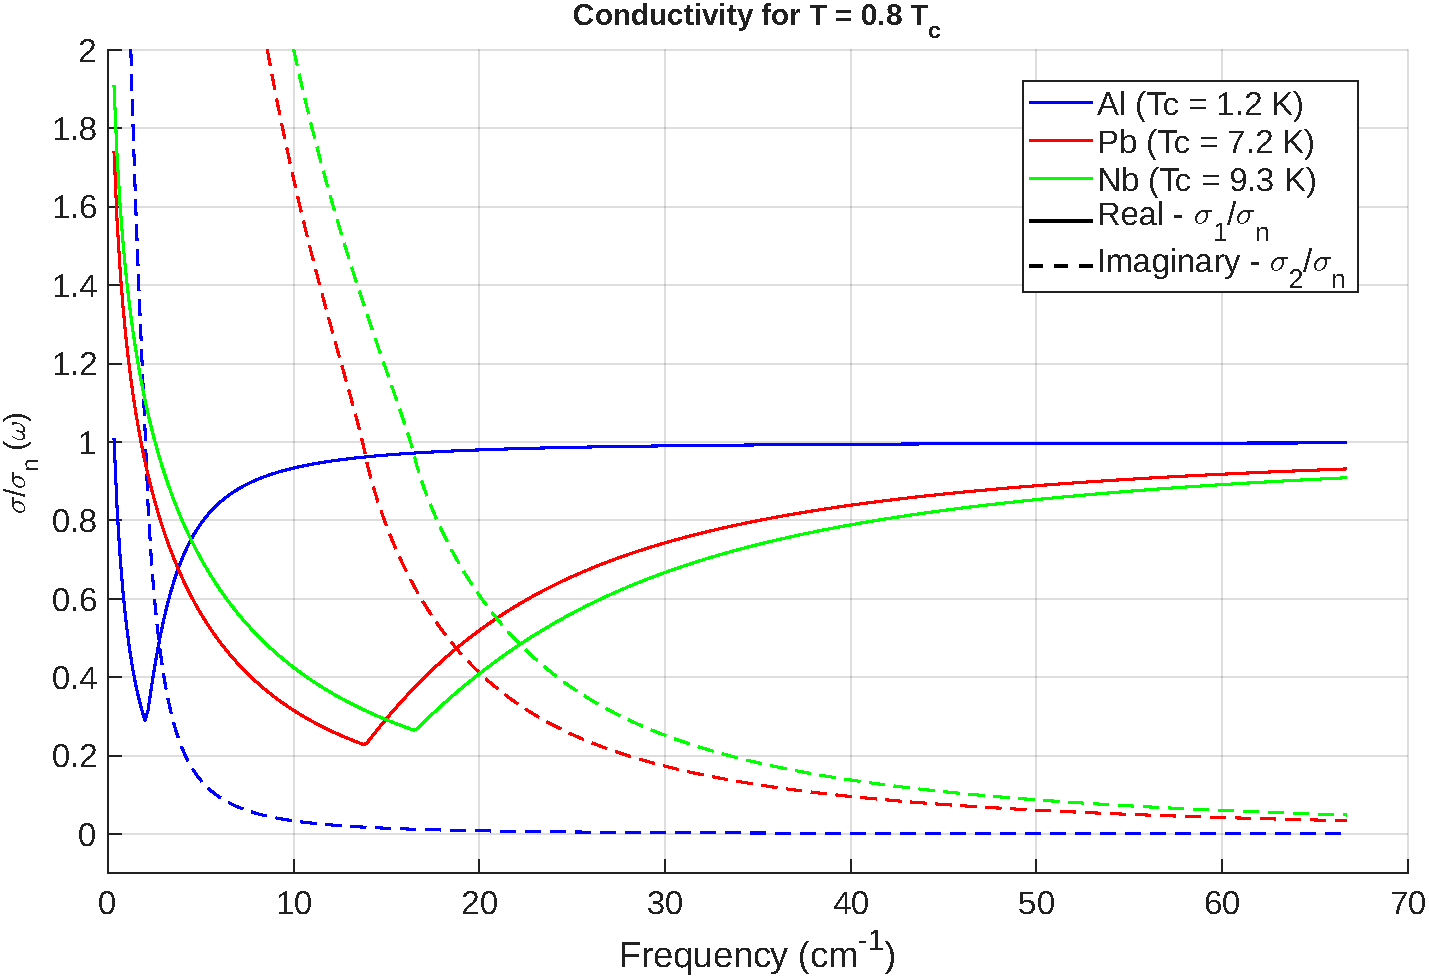
\includegraphics[width=0.8\textwidth]{../Immages/BCS_Comparison_0.8Tc.pdf}
    \caption{Complex conductivity for different materials.}
     \label{fig:figura_cond_comparison}
\end{figure}

\begin{figure}[!h]
    \centering
    % Sotto-figura di SINISTRA
    \begin{subfigure}[b]{0.49\textwidth}
        \centering
        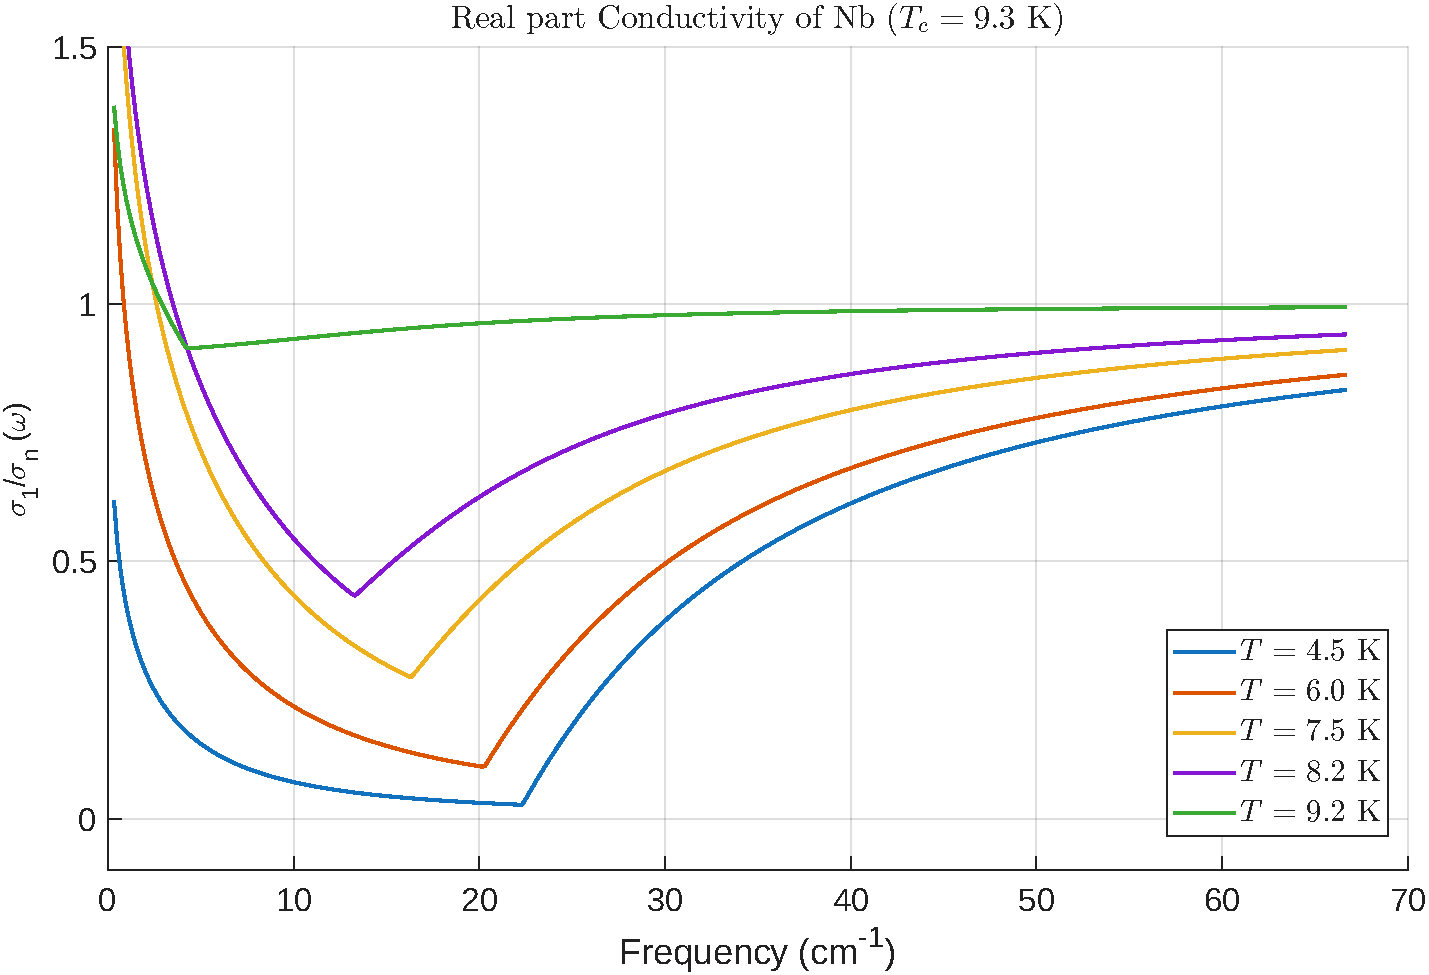
\includegraphics[width=\textwidth]{../Immages/BCS_Nb_real_cond_diffT_conv_units.pdf}
        %\caption{Didascalia dell'immagine a sinistra.}
        \label{fig:sinistra_Nb}
    \end{subfigure}
   \hfill
    % Sotto-figura di DESTRA
    \begin{subfigure}[b]{0.49\textwidth}
        \centering
        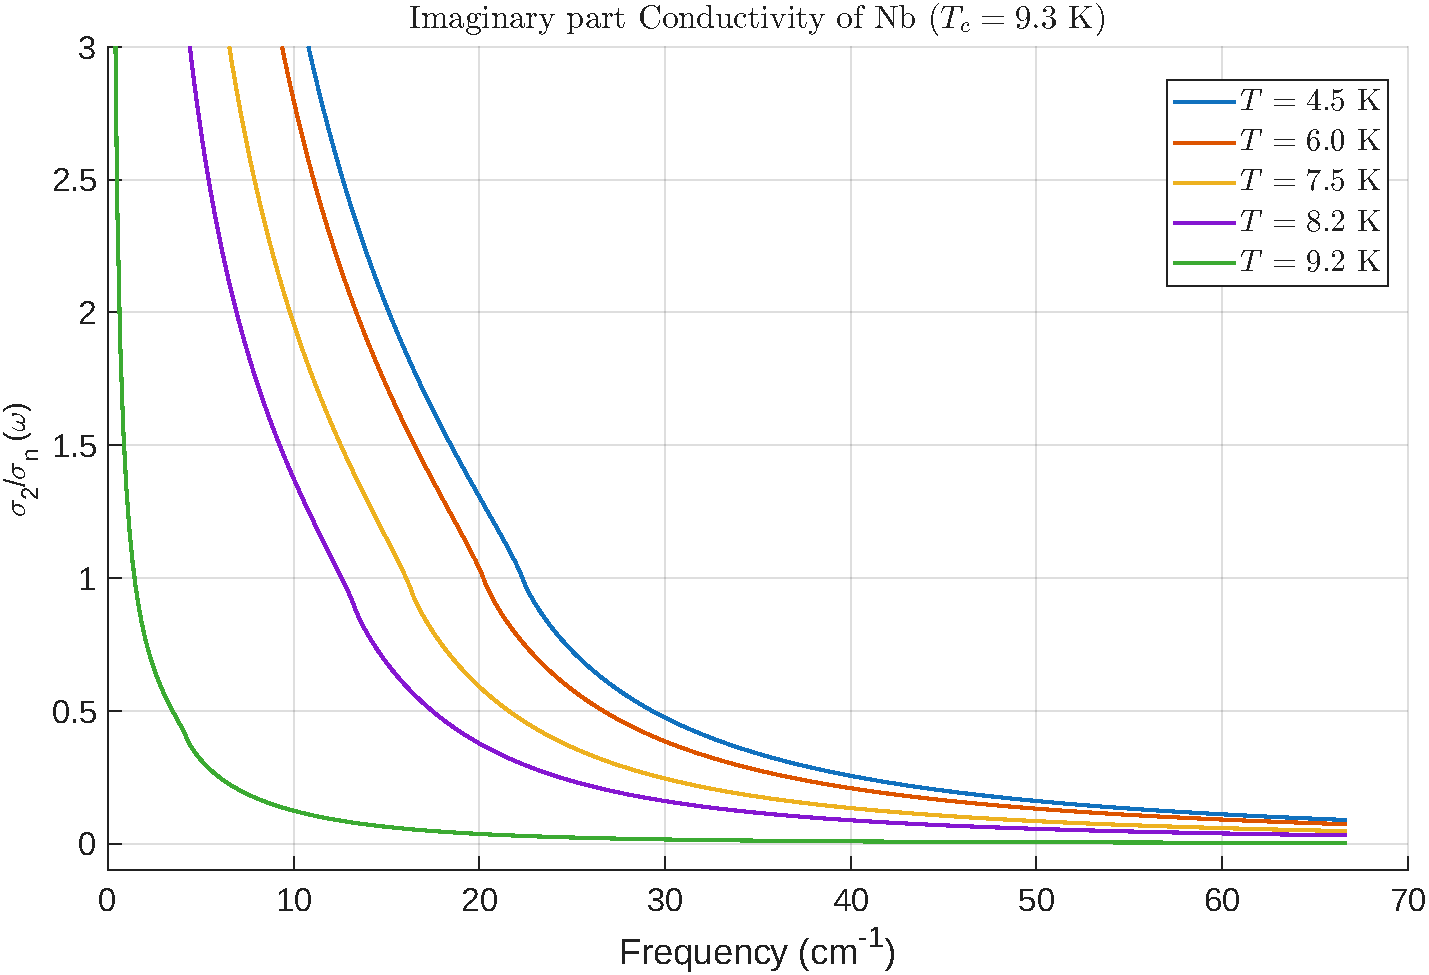
\includegraphics[width=\textwidth]{../Immages/BCS_Nb_imm_cond_diffT_conv_units.pdf}
        %\caption{Didascalia dell'immagine a destra.}
        \label{fig:destra_Nb}
    \end{subfigure}
    
    % Didascalia e Label GENERALI di tutta la figura
    \caption{Real (sx) and imaginary (dx) conductivity for Nb.}
    \label{fig:figura_completa_Nb}
\end{figure}


\begin{figure}[!h]
    \centering
    % Sotto-figura di SINISTRA
    \begin{subfigure}[b]{0.49\textwidth}
        \centering
        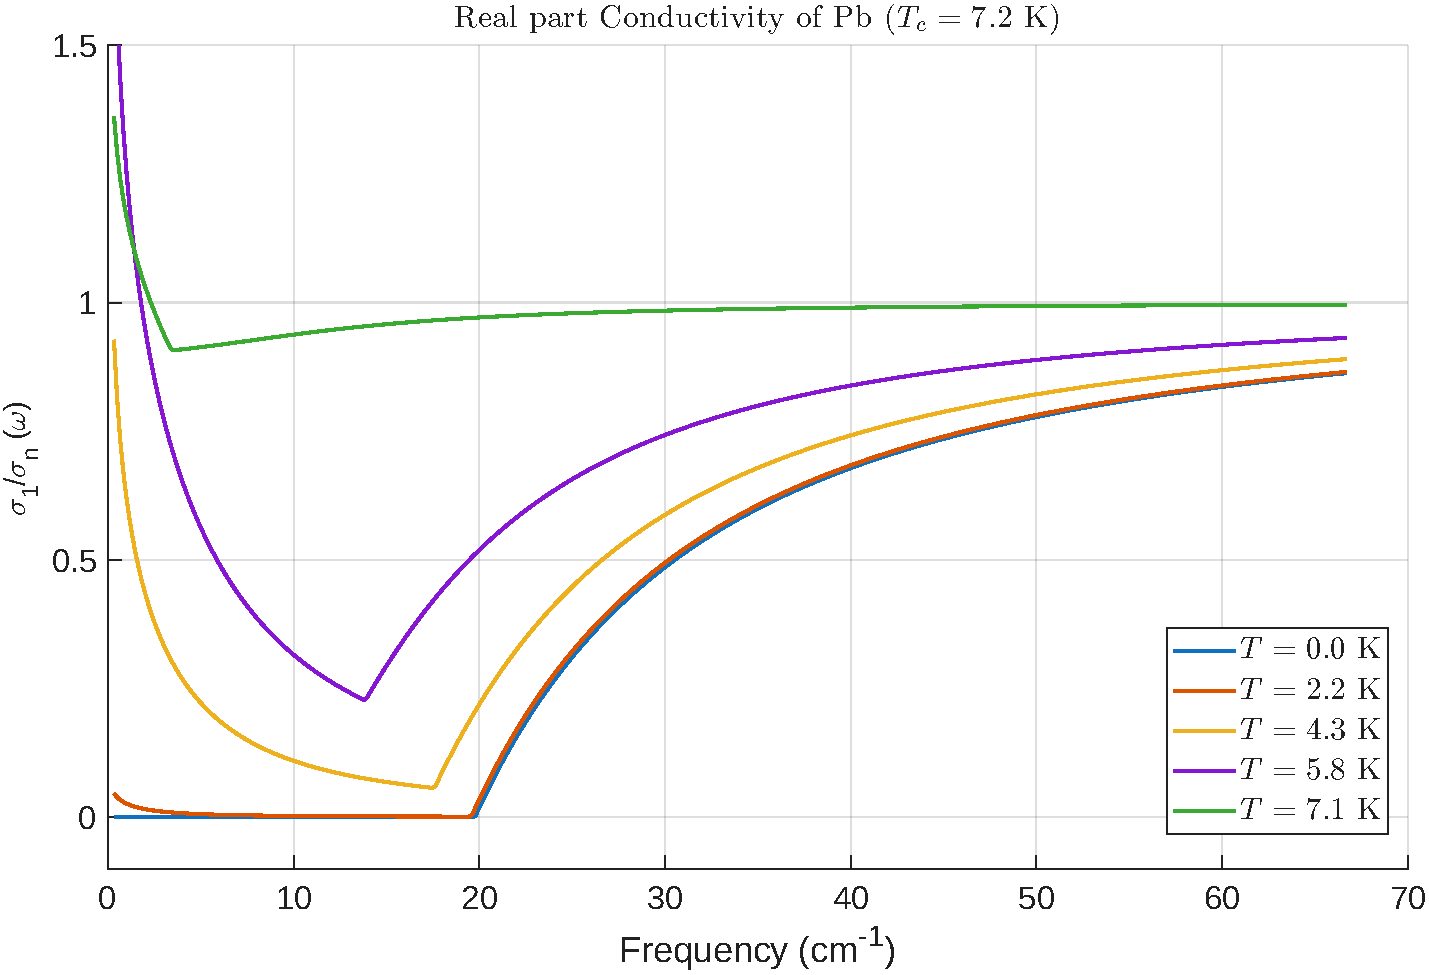
\includegraphics[width=\textwidth]{../Immages/BCS_Pb_real_cond_diffT_conv_units.pdf}
        %\caption{Didascalia dell'immagine a sinistra.}
        \label{fig:sinistra_Pb}
    \end{subfigure}
   \hfill
    % Sotto-figura di DESTRA
    \begin{subfigure}[b]{0.49\textwidth}
        \centering
        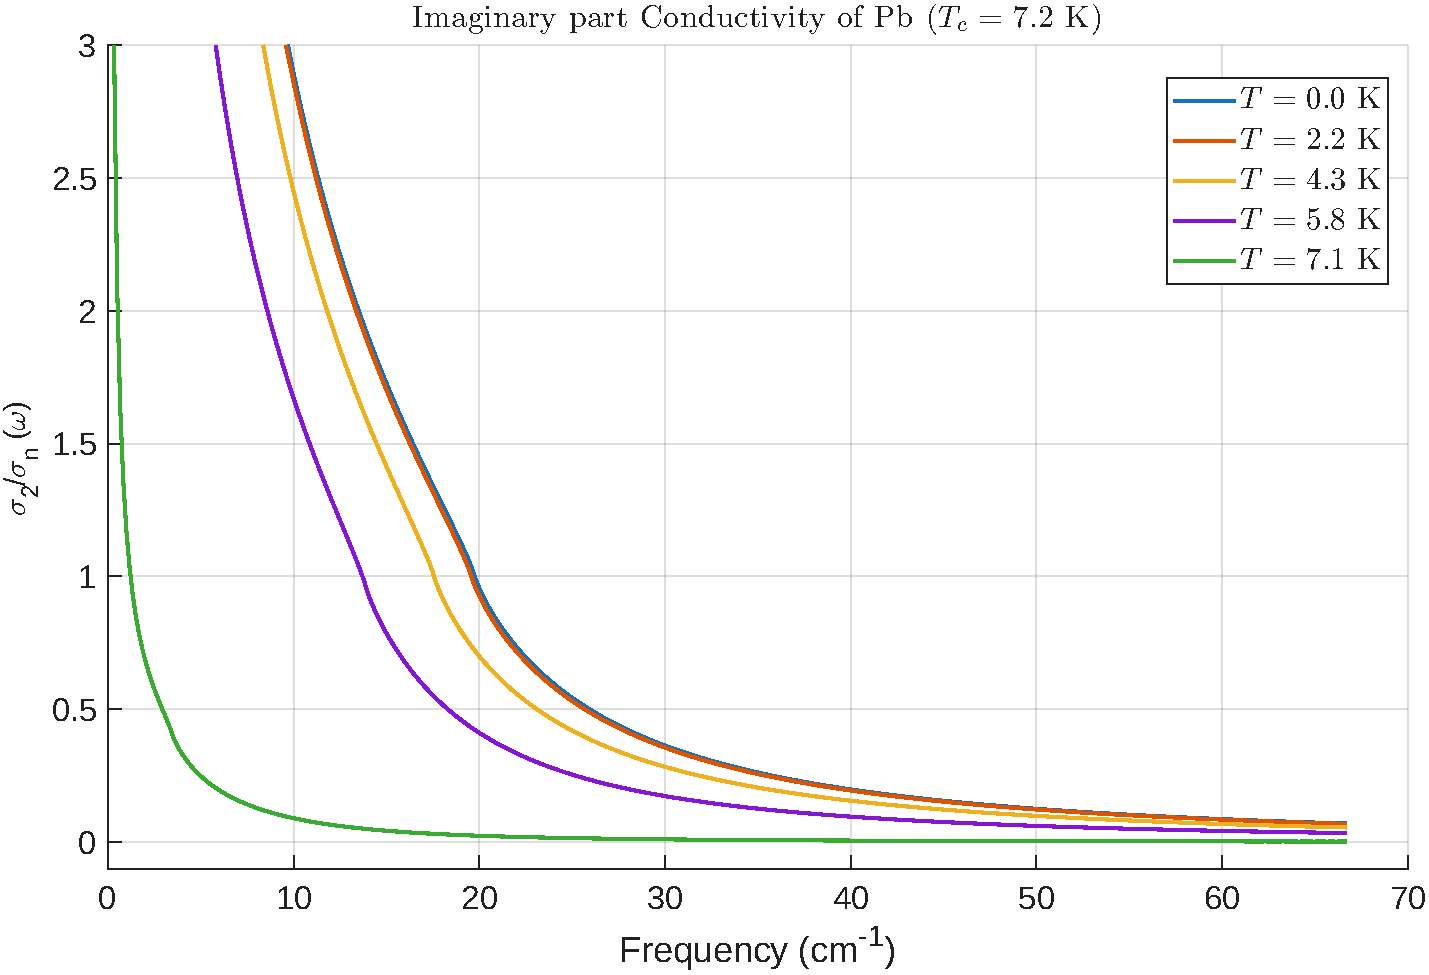
\includegraphics[width=\textwidth]{../Immages/BCS_Pb_imm_cond_diffT_conv_units.pdf}
        %\caption{Didascalia dell'immagine a destra.}
        \label{fig:destra_Pb}
    \end{subfigure}
    
    % Didascalia e Label GENERALI di tutta la figura
    \caption{Real (sx) and imaginary (dx) conductivity for Pb.}
    \label{fig:figura_completa_Pb}
\end{figure}


\begin{figure}[!h]
    \centering
    % Sotto-figura di SINISTRA
    \begin{subfigure}[b]{0.49\textwidth}
        \centering
        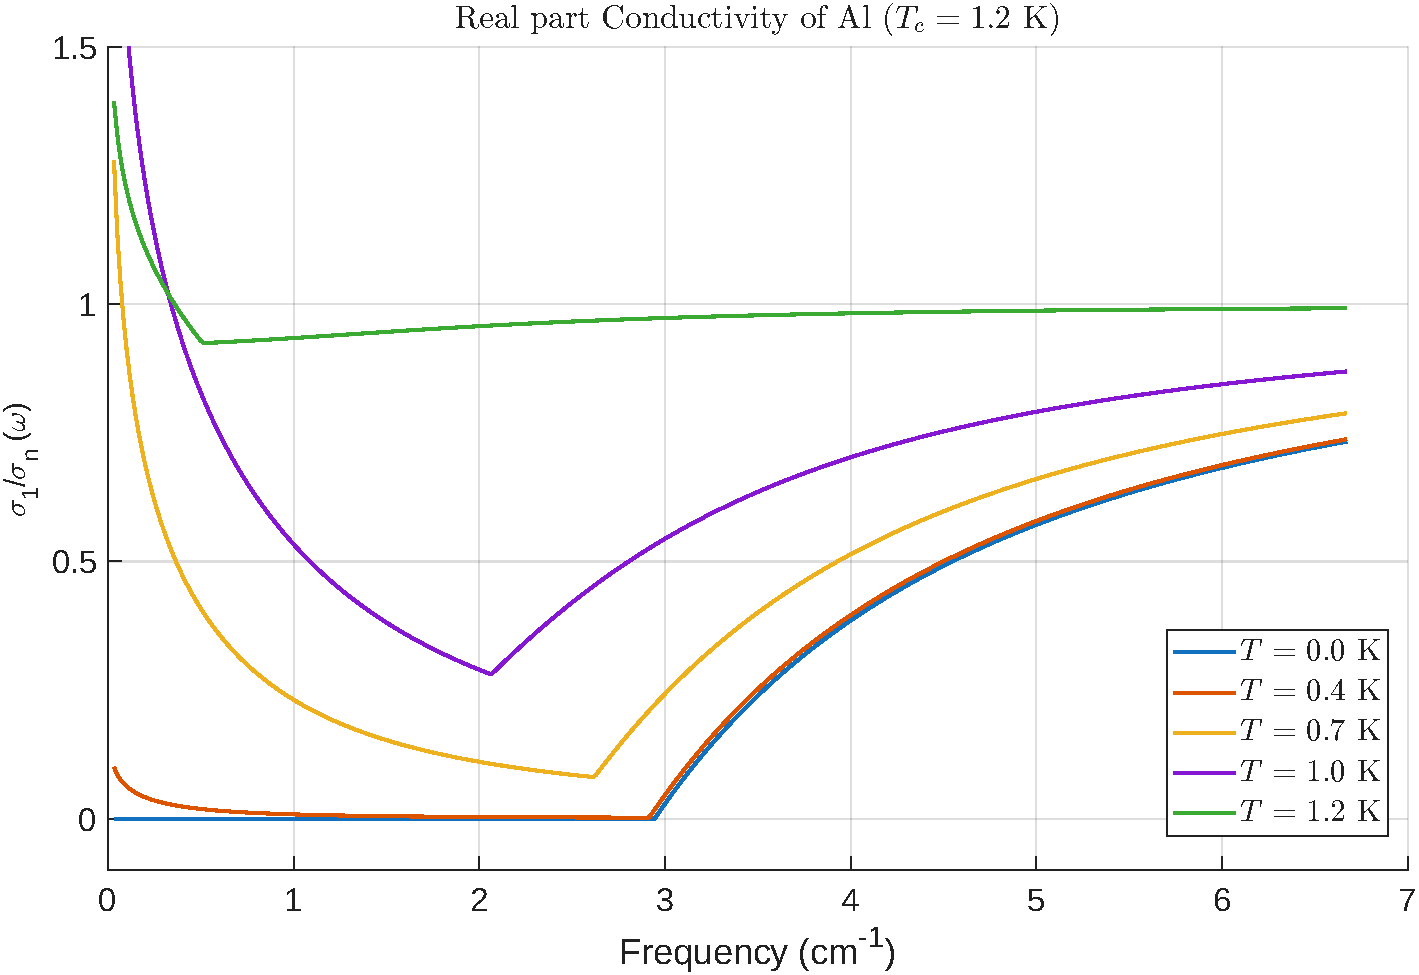
\includegraphics[width=\textwidth]{../Immages/BCS_Al_real_cond_diffT_conv_units.pdf}
        %\caption{Didascalia dell'immagine a sinistra.}
        \label{fig:sinistra_Al}
    \end{subfigure}
    \hfill
    % Sotto-figura di DESTRA
    \begin{subfigure}[b]{0.49\textwidth}
        \centering
        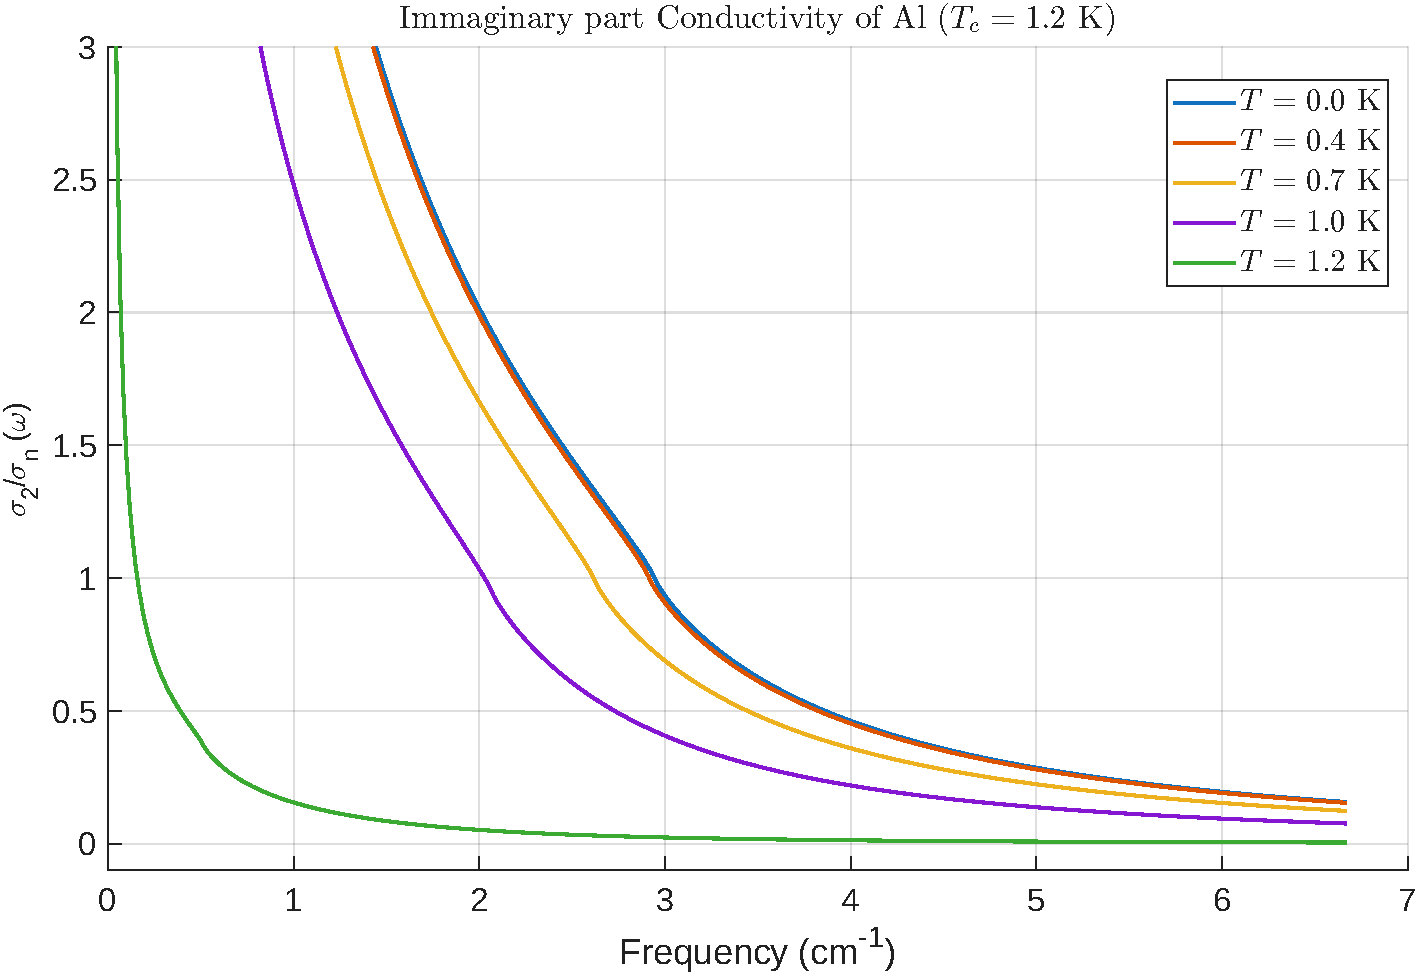
\includegraphics[width=\textwidth]{../Immages/BCS_Al_imm_cond_diffT_conv_units.pdf}
        %\caption{Didascalia dell'immagine a destra.}
        \label{fig:destra_Al}
    \end{subfigure}
    
    % Didascalia e Label GENERALI di tutta la figura
    \caption{Real (sx) and imaginary (dx) conductivity for Al.}
    \label{fig:figura_completa_Al}
\end{figure}

\begin{figure}[!h]
    \centering
    % Sotto-figura di SINISTRA
    \begin{subfigure}[b]{0.49\textwidth}
        \centering
        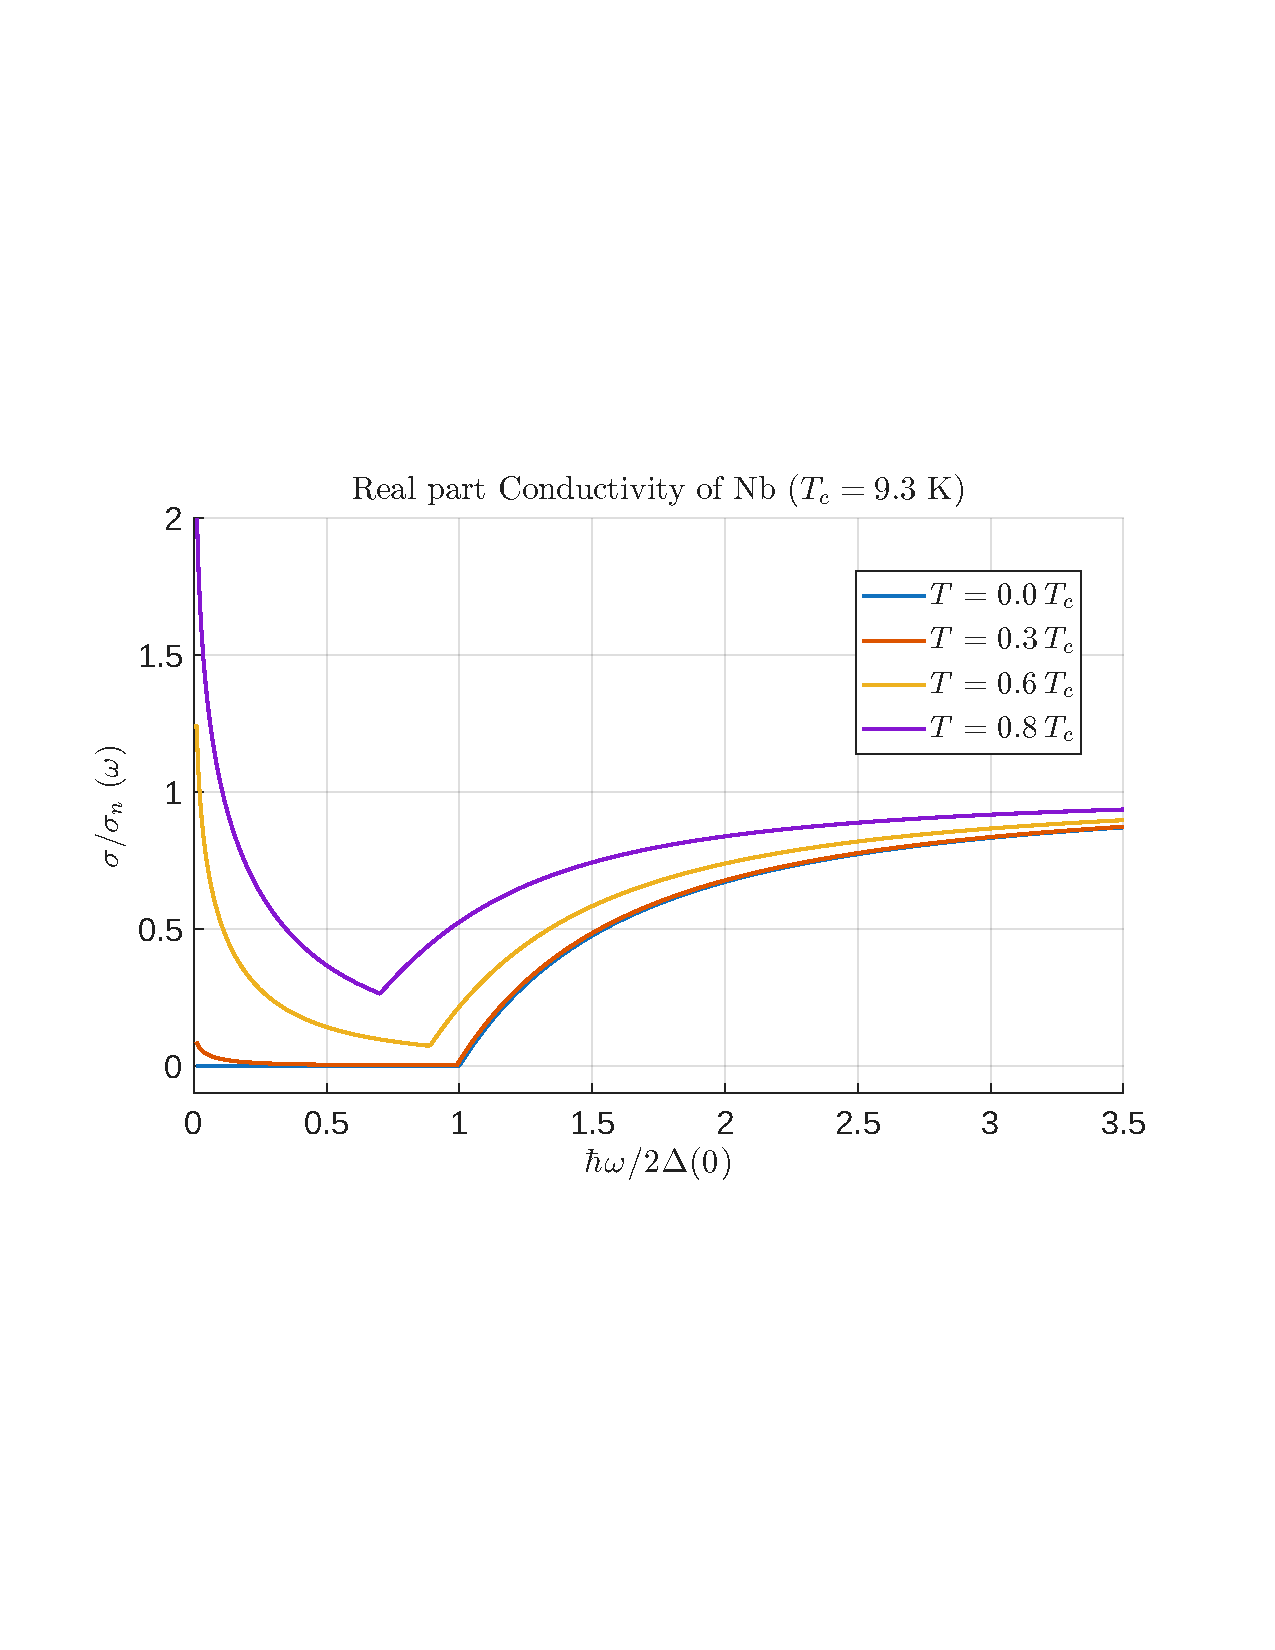
\includegraphics[width=\textwidth]{../Immages/BCS_Nb_real_cond_diffT.pdf}
        %\caption{Didascalia dell'immagine a sinistra.}
        \label{fig:sinistra_Nb_norm}
    \end{subfigure}
    \hfill
    % Sotto-figura di DESTRA
    \begin{subfigure}[b]{0.49\textwidth}
        \centering
        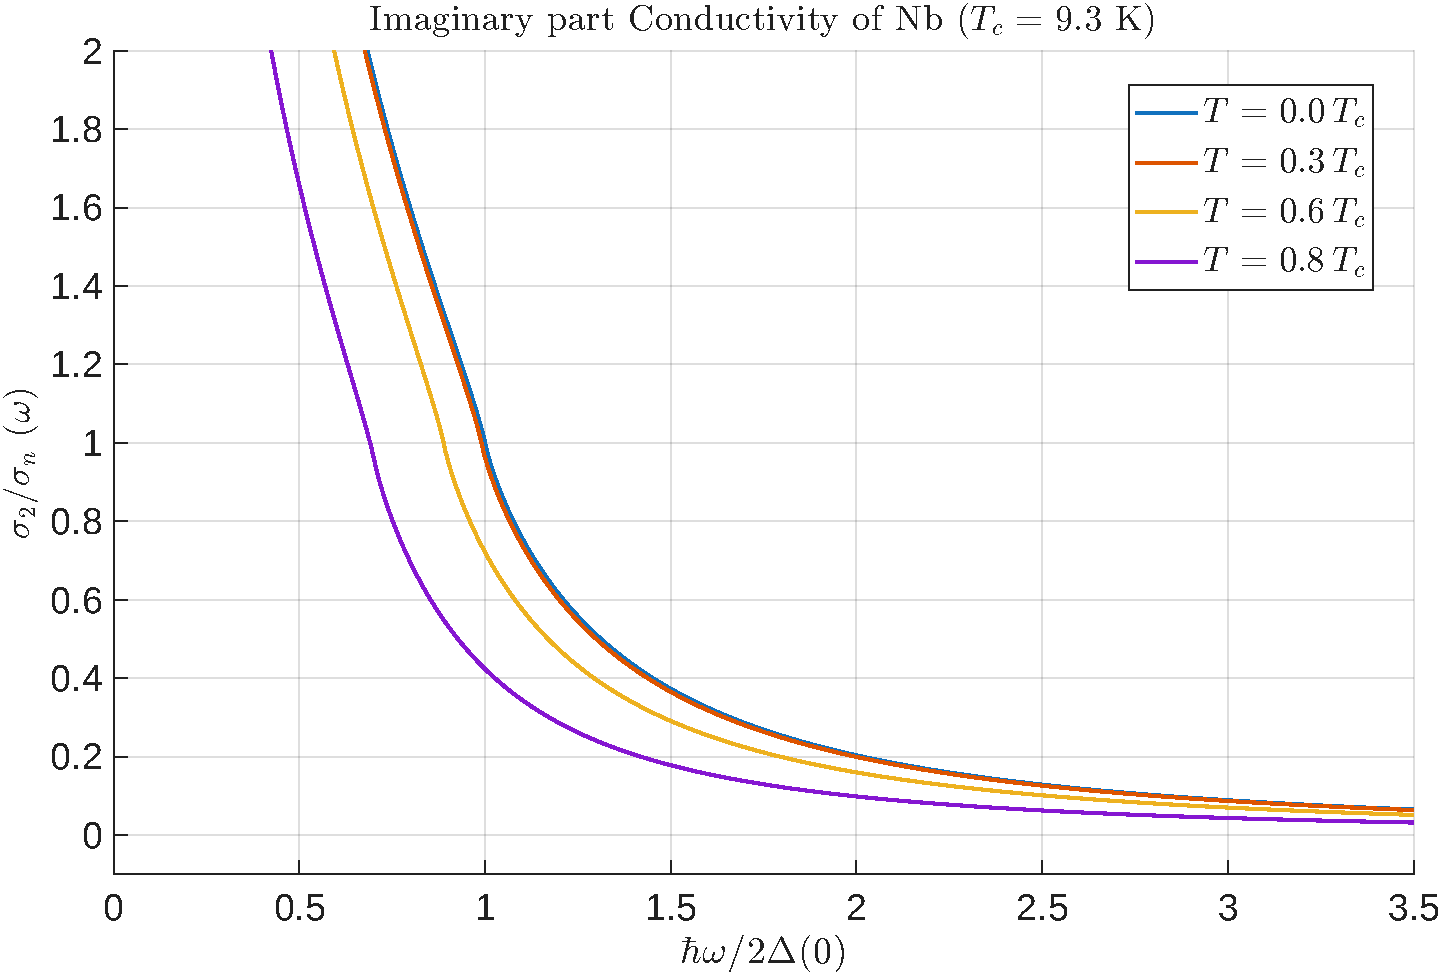
\includegraphics[width=\textwidth]{../Immages/BCS_Nb_imm_cond_diffT.pdf}
        %\caption{Didascalia dell'immagine a destra.}
        \label{fig:destra_Nb_norm}
    \end{subfigure}
    
    % Didascalia e Label GENERALI di tutta la figura
    \caption{Real (sx) and imaginary (dx) conductivity for Nb in normalized units, to check the gap corresponds at $T=0$.}
    \label{fig:figura_completa_Nb_norm}
\end{figure}


To evaluate the performances of the code that i've written, i compare the numerical solutions
with experimental data of Nb. To extract the data points from the figure i have used the online tool \texttt{WebPlotDigitizer}.
The results are showed in the Fig.\ref{fig:figura_completa_Nb_fit} below with $T_c=8.3$~K and $\alpha=4.1$.
\begin{figure}[!h]
    \centering
    % Sotto-figura di SINISTRA
    \begin{subfigure}[b]{0.49\textwidth}
        \centering
        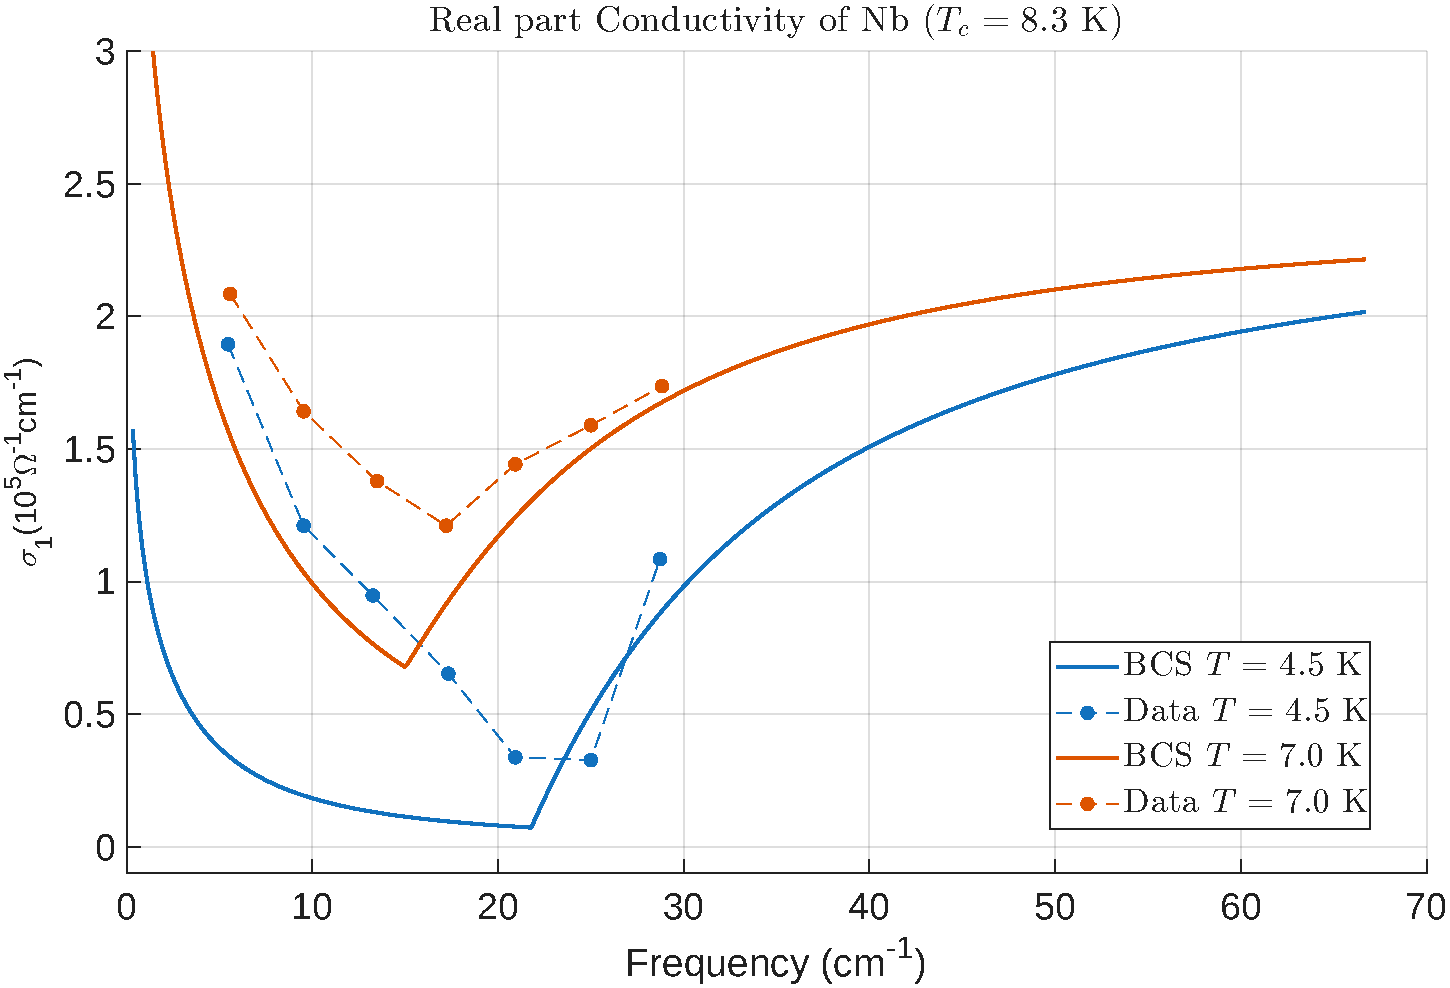
\includegraphics[width=\textwidth]{../Immages/BCS_Nb_real_cond_diffT_conv_units_fitexp.pdf}
        %\caption{Didascalia dell'immagine a sinistra.}
        \label{fig:sinistra_Nb_fit}
    \end{subfigure}
    \hfill
    % Sotto-figura di DESTRA
    \begin{subfigure}[b]{0.49\textwidth}
        \centering
        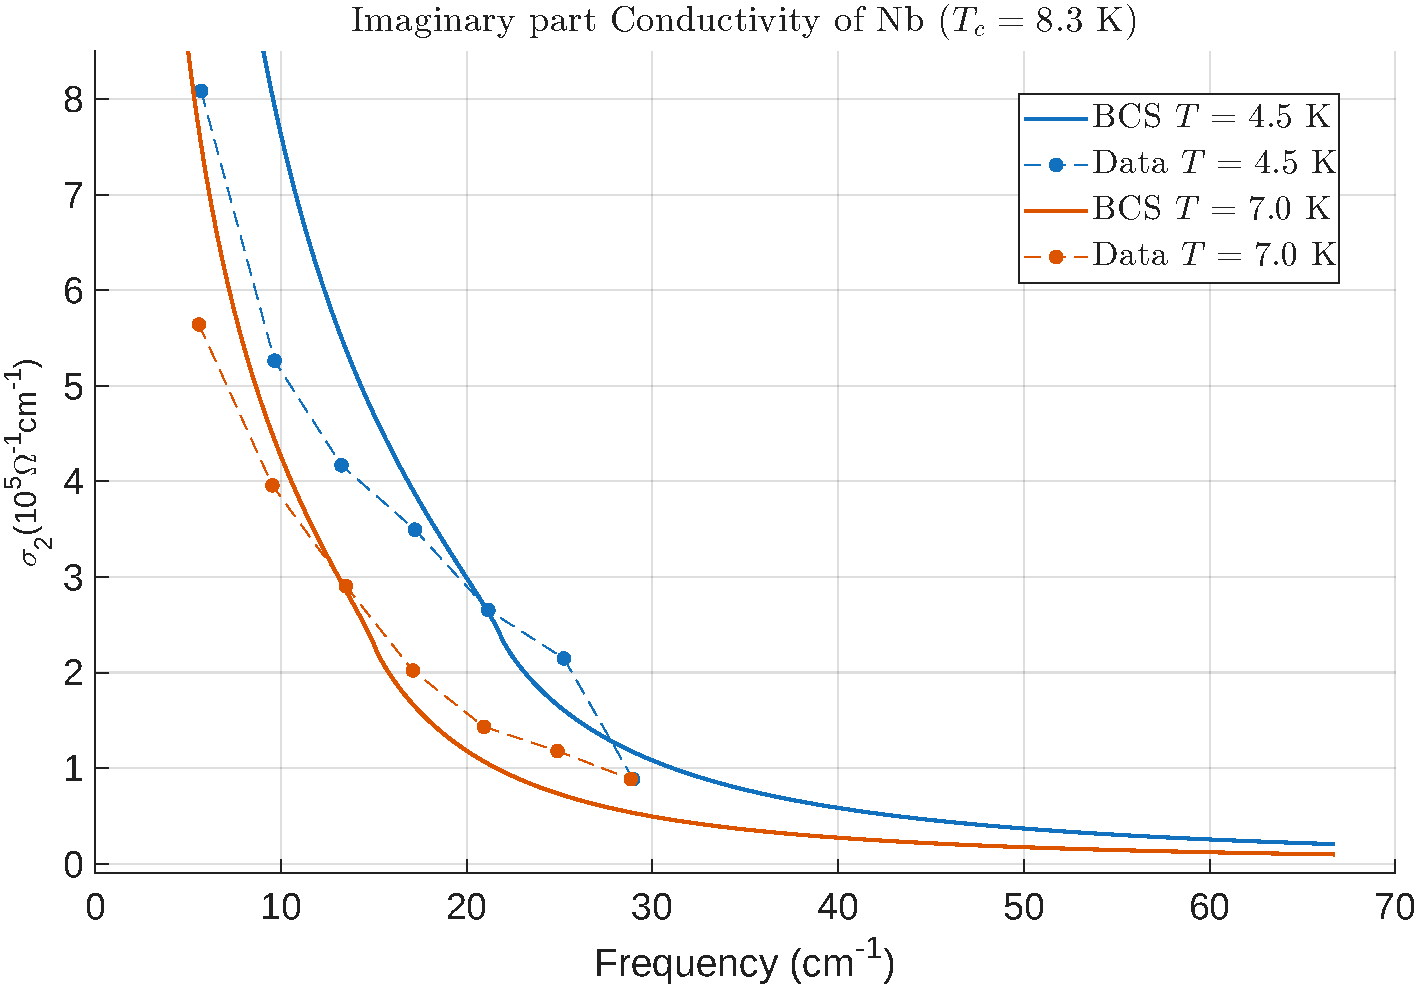
\includegraphics[width=\textwidth]{../Immages/BCS_Nb_imm_cond_diffT_conv_units_fitexp.pdf}
        %\caption{Didascalia dell'immagine a destra.}
        \label{fig:destra_Nb_fit}
    \end{subfigure}
    
    % Didascalia e Label GENERALI di tutta la figura
    \caption{Real (sx) and imaginary (dx) conductivity for Nb compared with experimental data.}
\label{fig:figura_completa_Nb_fit}
\end{figure}
We can see that the BCS understimates the value of the real conductivity $\sigma_1$, expecially for lower $T$, but we espected this for Niobium because is a strong-coupling
superconducting material while BCS is a weak-coupling theory ($\alpha = 3.65$). 

Another comparison that needs to be done is the one between the values of $\Delta$ at different temperatures extracted 
by the experimental data of conductivity, and the BCS mean field approximation used for the gap function in Eq.~\ref{eq:BCS_gap_approx}. The value of $2\Delta(T)$
is given by the frequency that corresponds to the minimum of the $\sigma_1$ at given temperature.
This is showed in Fig.~\ref{fig:Gap_comparison}. Furthermore in Fig.~\ref{fig:Gap_comparison} i have plotted the frequency at the minimum of $\sigma_1$ obtained
from the numerical solution of Eq.\ref{eq:MB-real_cond}, as a double check for the code.

\begin{figure}[!h]
    \centering
    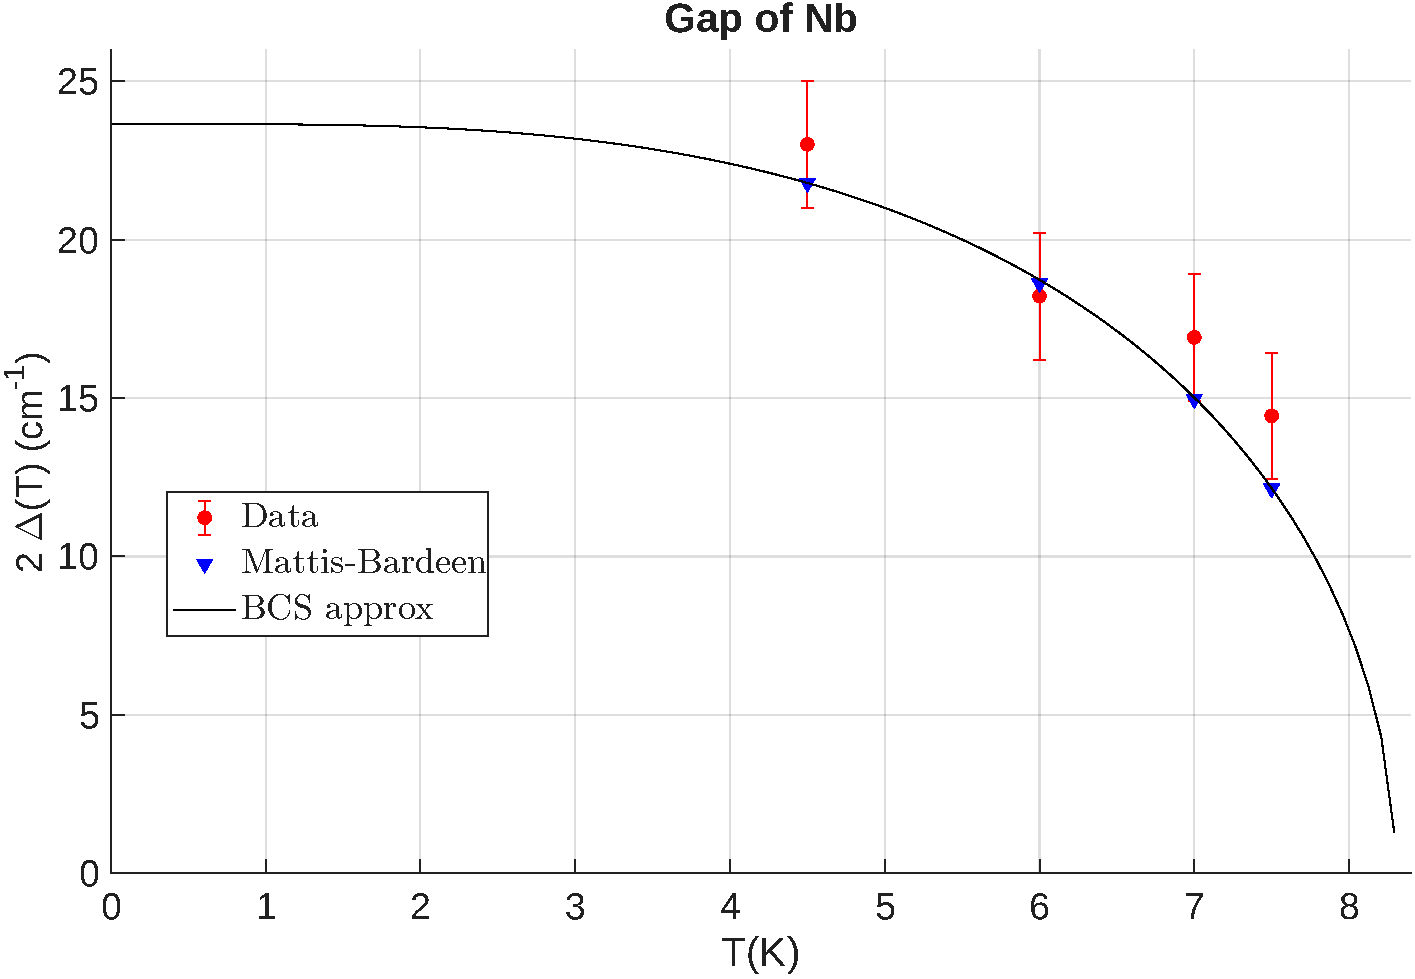
\includegraphics[width=0.7\textwidth]{../Immages/BCS_Gap_MB_vs_T_fitexp.pdf}
    \caption{Comparison between BCS approximation of $\Delta(T)$ and the values of $\Delta$ extracted by the data. Errorbars are $2~\text{cm}^{-1}$ from the paper [ref].}
\label{fig:Gap_comparison}
\end{figure}

\end{document}